\chapter{Question 2}
\label{question-2}
\section{Question}



\begin{itemize}
\item Ingest the 100 URIs from their resulting WARC files into a SOLR instance.
\begin{itemize}
\item  see the code + tutorial at:  \hyperref[savePage]{https://github.com/ukwa/webarchive-discovery}
\end{itemize}
\item Demonstrate several functioning queries on the files (a full front-end is not required)
\begin{itemize}
\item  describe the configuration choices you made in setting up SOLR and processing the documents	
\end{itemize}
\end{itemize}

\section{Solution}
\begin{itemize}
\item For setting up SOLR I used the link as provided in the question.
\item The instructions provided were clear and concise which helped me set-up the necessary tools without any issues.
\item Though I faced an issue when the pywb was running and I wouldn't be able to run SOLR. Then I realized that both the applications were trying to run on the same port as it was already in use. Upon closing the pywb instance and then running SOLR everything was working like a well oiled machine.
\item I merged all the WARC files that I had retrieved using wget, using the tool WARCMerge located at \hyperref[savePage]{https://github.com/maturban/WARCMerge}.
\item After merging the WARC file I ran the command for indexing as provided in the user instructions by the author of the tool.
\item Following this I ran the default web interface for SOLR and ran the following queries as displayed below.
\end{itemize}
\newpage
\begin{minipage}{\linewidth}
	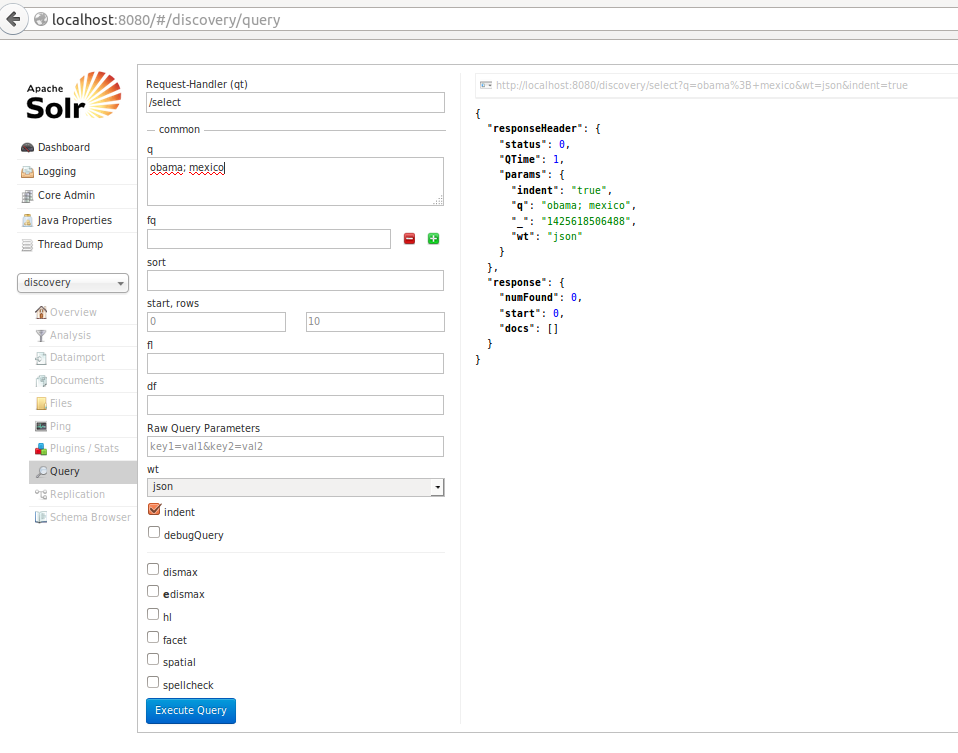
\includegraphics[scale=0.55]{figures/query/query_obama_mexico.PNG}
	\captionof{figure}{Query: obama; mexico}
	\label{query_obama_mexico}
\end{minipage}
\newpage
\begin{minipage}{\linewidth}
	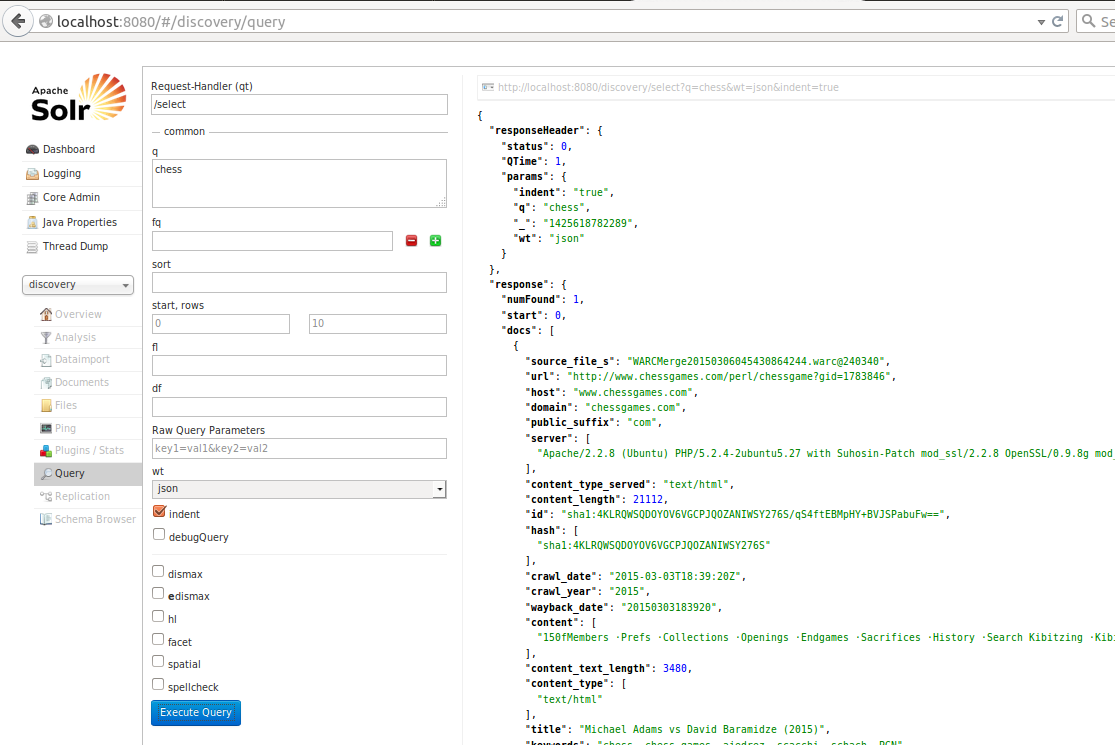
\includegraphics[scale=0.55]{figures/query/query_chess.PNG}
	\captionof{figure}{Query: chess}
	\label{query_chess}
\end{minipage}

\begin{minipage}{\linewidth}
	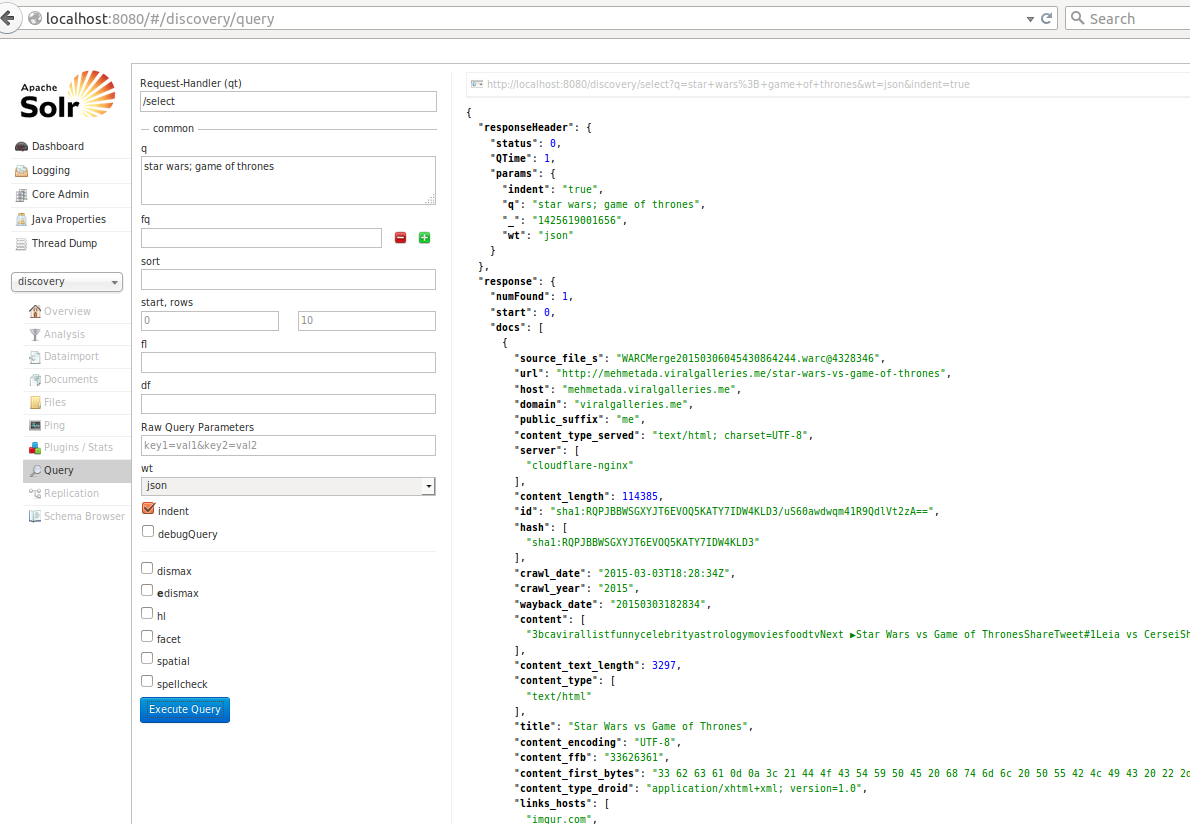
\includegraphics[scale=0.55]{figures/query/query_star_wars_game_of_thrones.PNG}
	\captionof{figure}{Query: star wars; game of thrones}
	\label{query_star_wars_game_of_thrones}
\end{minipage}
\begin{itemize}
\item From the previous query I toggled the case for the search parameter and the ranking of the results is modified as shown below.
\newpage
\begin{minipage}{\linewidth}
	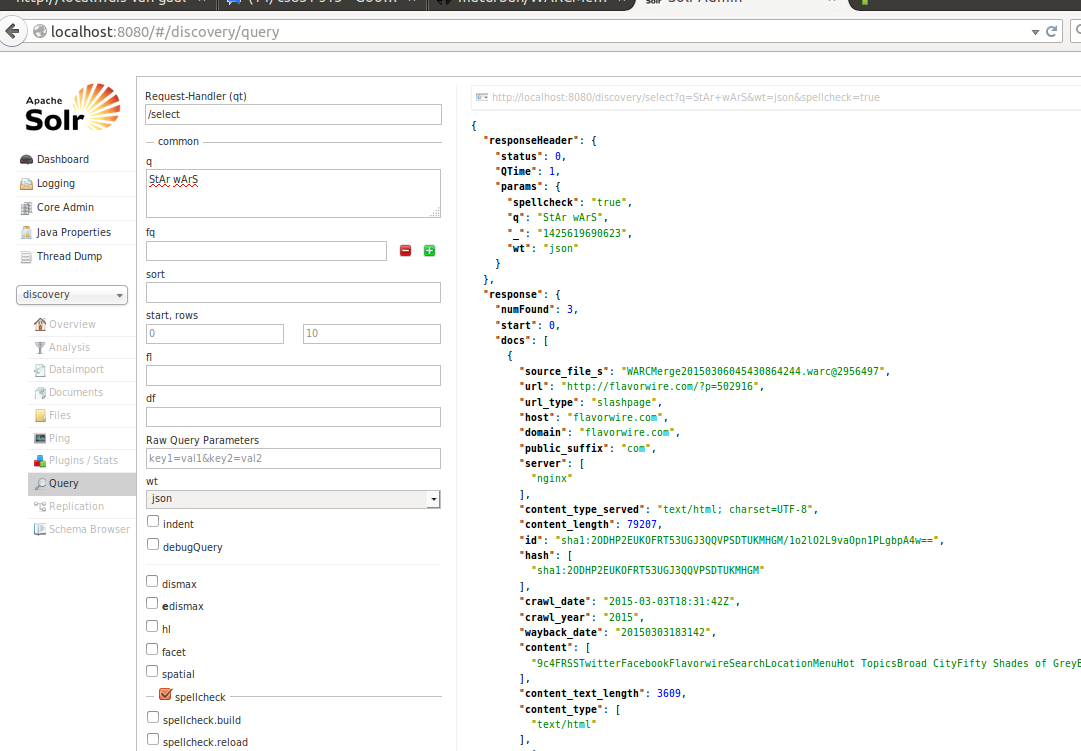
\includegraphics[scale=0.55]{figures/query/query_star_wars.PNG}
	\captionof{figure}{Query: StAr wArS}
	\label{query_chess}
\end{minipage}
\end{itemize}